\label{chap:methods}
This chapter describes the design and implementation of a system that simultaneously acquires EMG and EDA signals from a single muscle site, with galvanic isolation as the central design requirement.
\section{Design Specifications}
%What the system needs
The system was designed to simultaneously acquire EMG and EDA signals from a single muscle site and digitize them using a National Instruments USB-6356 data acquisition card. The specifications common to both acquisition channels are summarized in Table~\ref{tab:design_specs}.

\begin{table}[h]
\centering
\caption{System-level design specifications.}
\label{tab:design_specs}
\begin{tabular}{l l}
\toprule
\textbf{Parameter}         & \textbf{Value} \\
\midrule
Supply voltage             & \SI{5}{\volt} (USB-C) \\
Sampling rate              & \SI{2}{\kilo\hertz} per channel \\
ADC resolution             & 16-bit \\
ADC input range            & \SI{\pm 2}{\volt} \\
Number of channels         & 2 (EMG and EDA) \\
Target EMG bandwidth       & \SI{10}{\hertz}-\SI{500}{\hertz} \\
Target EDA bandwidth       & \SI{0}{\hertz}-\SI{5}{\hertz} \\
Galvanic isolation         & Required between EMG and EDA front-ends \\
\bottomrule
\end{tabular}
\end{table}


\section{System Architecture}
\label{sec:system_architecture}
%Here is the problem and our top-level solution
This section presents a high-level overview of a system designed to simultaneously measure electromyography (EMG) and electrodermal activity (EDA) at the same muscle site. The main hardware components are illustrated in Figure~\ref{fig:system_architecture} and include two dedicated front-end units for each modality (EMG and EDA), galvanic isolation stages, and a common data acquisition unit connected to a PC.

Each modality is equipped with its own set of surface electrodes placed over the target muscle. The raw signals are processed within their respective front-end units, where they are amplified and filtered according to their specific bandwidth and dynamic range. After conditioning, the signals from each front-end pass through an isolated amplifier stage that provides galvanic isolation. On the system side of the isolation barrier, the EMG and EDA channels are directed to separate analog input channels on the NI USB-6356. These channels are sampled simultaneously and transmitted to a PC for offline signal processing and analysis.

The power architecture operates on the same principle. A single \SI{5}{\volt} supply feeds two independent, isolated DC-DC converters, one for each front-end. This ensures that each front-end operates from its own isolated power supply and communicates with the data acquisition unit via its own signal isolation stage. The combination of power and signal isolation enables galvanic separation between the EMG and EDA front-ends, minimizing ground-loop interference and crosstalk between the two modalities while still permitting simultaneous data acquisition on a shared device. The following sections describe the implementation of each component in the order they appear in the signal chain.

\begin{figure}[H]
    \centering
    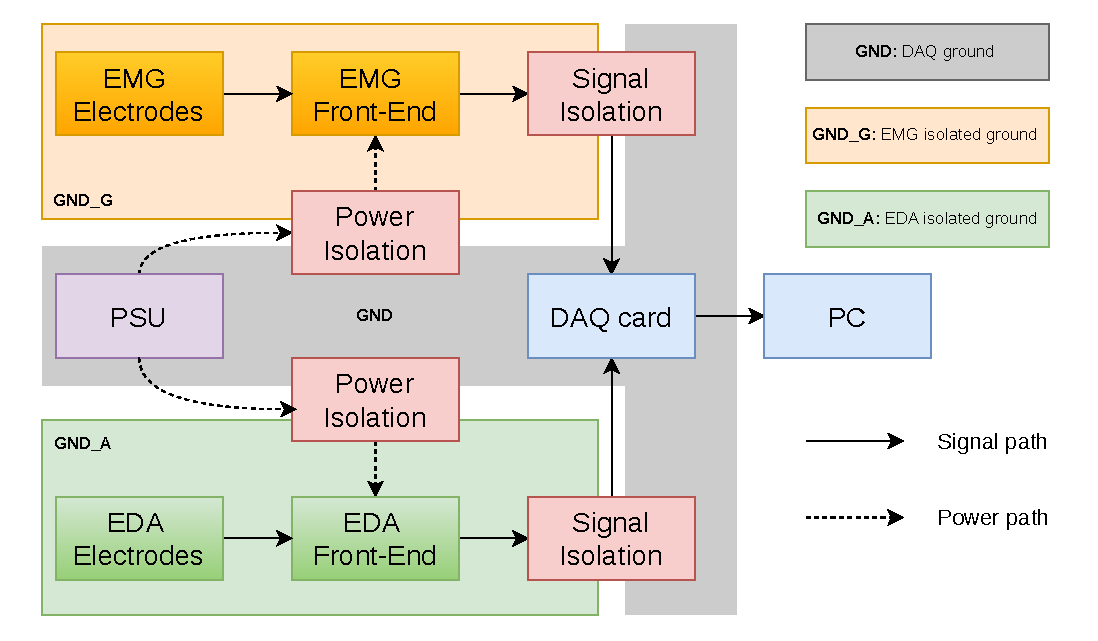
\includegraphics[width=\textwidth]{figures/system_architecture_gnd.drawio.pdf}
    \caption{System architecture of the simultaneous EMG and EDA acquisition system.}
    \label{fig:system_architecture}
\end{figure}

\section{Hardware Development}
%Describe how I implemented it
This section describes the implementation of the EMG and EDA front-ends and the galvanic isolation. In this work, the analog front-end is defined as the signal conditioning circuitry that runs from the measurement electrodes up to, but not including, the galvanic isolation stage.
The circuit was implemented on a custom four-layer printed circuit board (PCB), designed in KiCad and fabricated with help from ELAB at UiO.

\subsection{EMG Front-End}
\label{sec:EMG_frontend}
%Total gain = 733.3

%The component designators in the PCB layout differ from those in the schematic figures, as the schematic was redrawn for clarity.
The EMG front-end was based on the circuit proposed by \textcite{yang_detection_2020}, with all five stages redesigned for this implementation. From the electrodes, the signal passed through an instrumentation amplifier, a \SI{50}{\hertz} notch filter, a high-pass filter with an amplification stage, a Sallen-Key low-pass filter, and a voltage-lifting circuit. Each stage was powered by an isolated \SI{\pm 5}{\volt} dual rail from the TPS65133, described in Section~\ref{sec:EMG_power}. The resulting block diagram is shown in Fig.~\ref{fig:emg-frontend-blocks}.

%As mentioned in \ref{sec:sEMG_signal} the useful frequency contents spans from \SIrange{10}{500}{\hertz}, with amplitude from active contraction of the muscle at \SIrange{60}{300}{\micro\volt}.

%Split up the blocks
\begin{figure}[H]
    \centering
    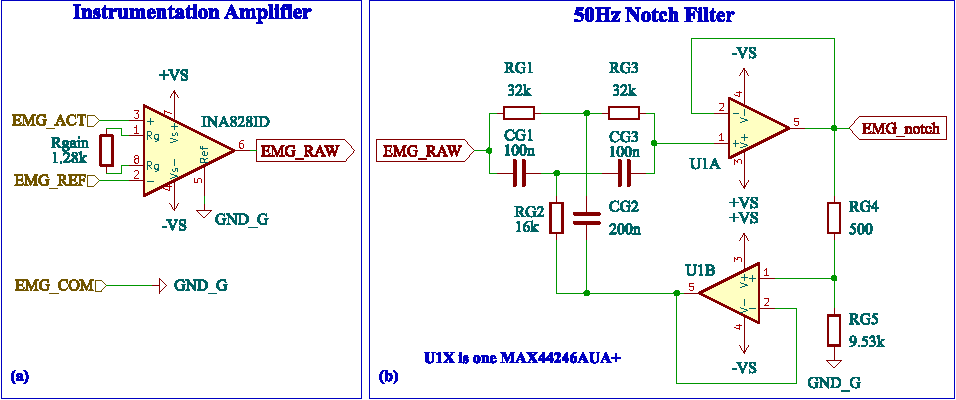
\includegraphics[width=\textwidth]{figures/version_2_figures-EMG building blocks 1 (cropped) (pdfresizer.com).pdf} \\
    \vspace{1mm}
    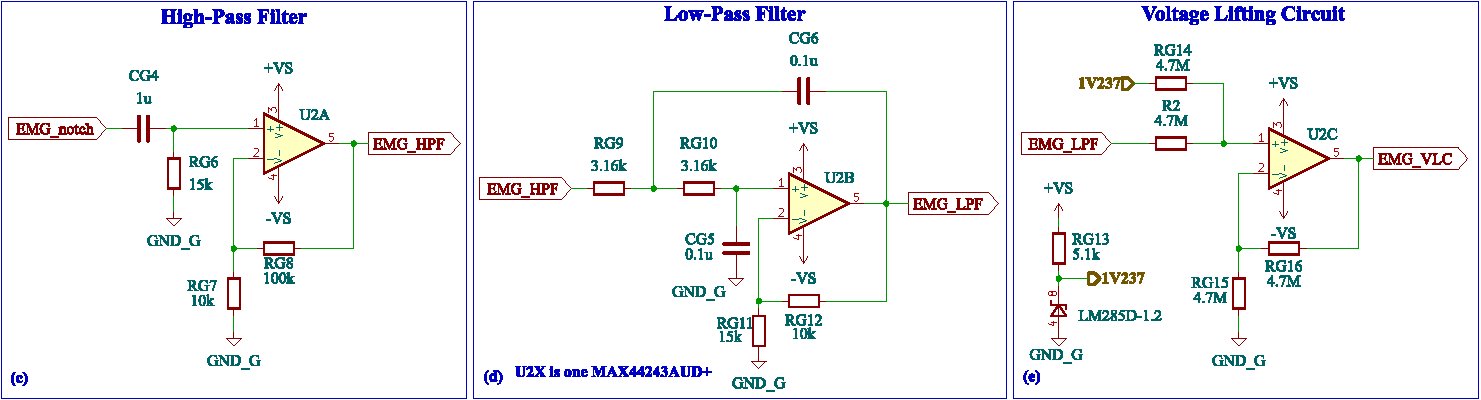
\includegraphics[width=\textwidth]{figures/version_2_figures-EMG building blocks 2 (cropped) (pdfresizer.com).pdf}
    \caption{EMG front-end building blocks. \textbf{(a)} Instrumentation amplifier. \textbf{(b)} 50Hz notch filter. \textbf{(c)} High-pass filter.\textbf{(d)} Low-pass filter. \textbf{(e)} Voltage Lifting Circuit. }
    \label{fig:emg-frontend-blocks}
\end{figure}

\subsubsection{Instrumentation Amplifier}
\label{sec:ina828}
The first stage was an INA828 instrumentation amplifier (Texas Instruments). Its CMRR of \SI{110}{\decibel} satisfied the \SI{80}{\decibel} minimum recommended for controlled isometric sEMG recordings~\cite{kamen_essentials_2010}. Gain was set to approximately \num{40} by connecting a \SI{1.28}{\kilo\ohm} resistor between the $R_G$ pins, following the relation given in the component datasheet~\cite{noauthor_ina828_nodate}:
\begin{equation}
    G = 1 + \frac{\SI{50}{\kilo\ohm}}{R_G}.
    \label{eq:ina828-gain}
\end{equation} 

\subsubsection{Analog Filter Chain}
After the instrumentation amplifier, the signal passed through three filter stages. The cutoff frequency for all passive RC stages was calculated using:
\begin{equation}
    f_c = \frac{1}{2\pi RC}.
    \label{eq:RC_fc}
\end{equation}

\paragraph{50\,Hz Notch Filter}
Power-line interference appears as a large, narrowband disturbance at \SI{50}{\hertz} in the European grid environment, since the sEMG signal contains useful spectral content on both sides of \SI{50}{\hertz}; therefore, a notch filter was preferred over simply raising the high-pass cutoff. 
A twin-T active notch topology was implemented, as shown in Figure \ref{fig:emg-frontend-blocks}b, with the notch frequency set to \SI{50}{\hertz} by the passive network values. The active feedback path, implemented using an operational amplifier, increased the notch's quality factor beyond what a passive twin-T alone could achieve.
The quality factor was determined from the simulated frequency response (Figure~\ref{fig:EMG_LTSpice_bode}):
\begin{equation}
    Q = \frac{f_0}{f_\text{upper} - f_\text{lower}} 
    = \frac{\SI{50}{\hertz}}{\SI{55.2}{\hertz} - \SI{44.7}{\hertz}} 
    \approx 5
    \label{eq:notch_q}
\end{equation}
where $f_\text{upper}$ and $f_\text{lower}$ are the upper and lower \SI{-3}{\decibel} frequencies from the Bode plot.

\paragraph{High-Pass Filter} %Gain = 11
\label{sec:EMG_hpf}
The high-pass stage consisted of a passive RC filter followed by a non-inverting operational amplifier. From Figure~\ref{fig:emg-frontend-blocks}c, components $CG4 = \SI{1}{\micro\farad}$ and $RG6 = \SI{15}{\kilo\ohm}$ set the cutoff frequency to $f_c = \SI{10}{\hertz}$ using Eq.~\ref{eq:RC_fc}, and components $RG7 = \SI{10}{\kilo\ohm}$ and $RG8 = \SI{100}{\kilo\ohm}$ set the amplifier gain to \num{11}.
The International Society for Electrophysiology and Kinesiology (ISEK) recommended a \SI{10}{\hertz} high-pass cutoff for sEMG recordings under controlled conditions, and \SI{20}{\hertz} for dynamic movements where motion artifacts were more pronounced~\cite{kamen_essentials_2010}. Since the protocol employed isometric contractions, \SI{10}{\hertz} was selected to retain the low-frequency spectral content associated with motor unit firing patterns~\cite{kamen_essentials_2010}.

\paragraph{Low-Pass Filter} %Gain = 5/3
\label{sec:EMG_lpf}
The final stage was a second-order Sallen-Key low-pass filter. When both resistors and both capacitors are equal, the cutoff frequency reduces to the same expression as a passive RC circuit, given by Eq.~\ref{eq:RC_fc}. From Fig.~\ref{fig:emg-frontend-blocks}d, components $CG5 = CG6 = \SI{0.1}{\micro\farad}$ and $RG9 = RG10 = \SI{3.16}{\kilo\ohm}$ gave a calculated cutoff of $f_c \approx \SI{500}{\hertz}$, the upper bandwidth limit of the sEMG spectrum~\cite{kamen_essentials_2010}. The filter gain was set to \num{1.67} by the feedback resistors $RG11 = \SI{15}{\kilo\ohm}$ and $RG12 = \SI{10}{\kilo\ohm}$, following $G = 1 + R_{G11}/R_{G12}$.The simulated cutoff was \SI{530}{\hertz}, as seen in Fig.~\ref{fig:EMG_LTSpice_bode}.


\subsubsection{Voltage Lifting Circuit} 
\label{sec:EMG_voltage_lifter}
A voltage-lifting circuit offsets the EMG output to a \SI{1.237}{\volt} midpoint, set by an LM285 precision voltage reference. The bipolar sEMG waveform was thereby centered within the DAQ input range, keeping both signal rails clear of clipping.

The output $EMG\_VLC$ was passed to the galvanic isolation stage, described in Section~\ref{sec:galvanic_isolation}.

\subsubsection{Total Chain Gain}
\label{sec:EMG_total_gain}
The total voltage gain was the product of the instrumentation amplifier gain and the filter chain gain:
\begin{equation}
    G_\text{total} = G_\text{INA828} \times G_\text{filters}
    =G_\text{INA828} \times (G_\text{HPF} \times G_\text{LPF})  =\num{40} \times \num{11} \times \num{1.67} \approx \num{733.3}.
    \label{eq:total-gain}
\end{equation}
At the maximum sEMG amplitude of \SI{300}{\micro\volt}, the front-end output reached approximately \SI{220}{\milli\volt}, well within the \SI{\pm5}{\volt} input range of the DAQ card. The Bode plot in Fig.~\ref{fig:EMG_LTSpice_bode} showed the simulated frequency response of the complete front-end.

\begin{figure}[H] 
    \centering
    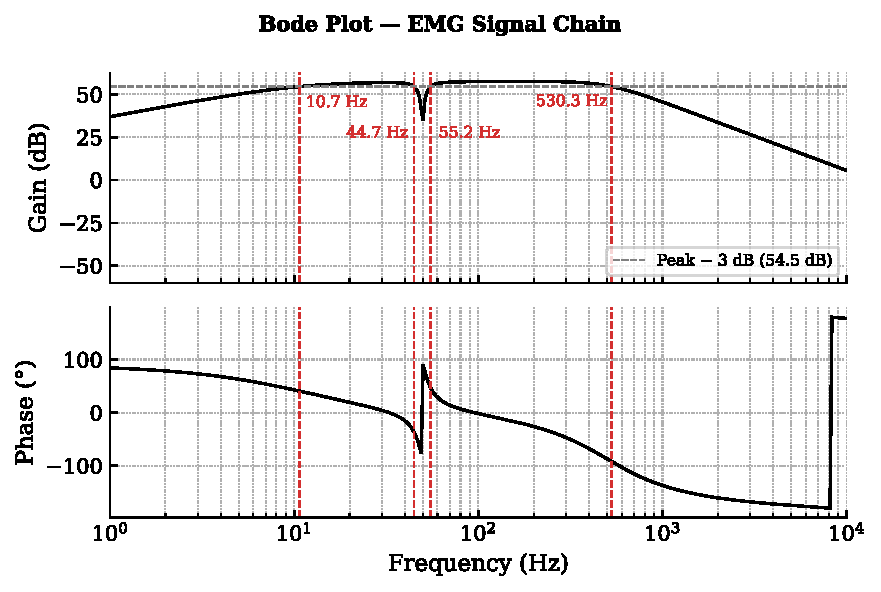
\includegraphics[width=\textwidth]{figures/EMG_LTSpice_bode.pdf}
    \caption{Simulated frequency response of the EMG front-end analog filter chain.  The passband spans \SIrange{10}{500}{\hertz}, with the \SI{50}{\hertz} notch visible as a narrow attenuation band. The simulated cutoff frequencies were \SI{10.7}{\hertz} for the high-pass stage and \SI{530}{\hertz} for the low-pass stage.}
    \label{fig:EMG_LTSpice_bode}
\end{figure}
%Transfer function

\subsection{EDA Front-End}
\label{sec:EDA_frontend}
The EDA front-end followed the design of \textcite{zangroniz_electrodermal_2017}, with all component values unchanged. The only difference was replacing the AD860x with the MAX44243AUD+, which was already used in the EMG front-end. Three stages made up the circuit: a virtual ground reference, a voltage-controlled current source, and a third-order low-pass filter. Power came from a \SI{3.3}{\volt} rail derived from the AMS1117-3.3, described in Section~\ref{sec:EDA_power}. The circuit is shown in Fig.~\ref{fig:EDA-frontend-blocks}.

\begin{figure}[H]
    \centering
    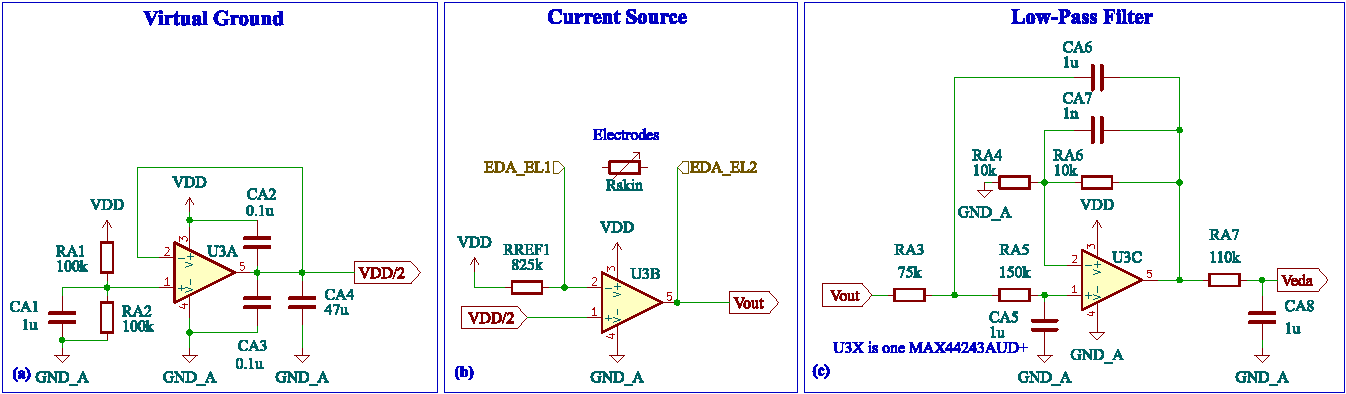
\includegraphics[width=\textwidth]{figures/version_2_figures-EDA Building Block (cropped) (pdfresizer.com).pdf}
    \caption{EDA front-end building blocks. \textbf{(a)} Virtual ground. \textbf{(b)} Current source. \textbf{(c)} Low-pass filter.}
    \label{fig:EDA-frontend-blocks}
\end{figure}

\subsubsection{Virtual Ground}
In a single-supply configuration, the op-amp has no negative rail, so a stable mid-supply reference is needed for the current source to operate correctly~\cite{zangroniz_electrodermal_2017}. A resistor divider ($R_{A1} = R_{A2} = \SI{100}{\kilo\ohm}$) split the \SI{3.3}{\volt} supply to give \SI{1.65}{\volt}, buffered by op-amp U3A to hold a low-impedance reference at the non-inverting input of U3B, as shown in Fig.~\ref{fig:EDA-frontend-blocks}a. $C_{A1}$ formed a low-pass filter with the divider impedance to keep supply noise off the reference node. $C_{b1}$, $C_{b2}$, and $C_b$ bypassed the \SI{3.3}{\volt} rail.

\subsubsection{Current Source}
\label{sec:EDA_current_source}
The reference resistor $R_{ref1}$ and the virtual ground voltage work together to determine the current injected into the skin~\cite{zangroniz_electrodermal_2017}:

\begin{equation}
    I_{skin} = \frac{1}{2}\frac{V_{DD}}{R_{ref}}
    \label{eq:EDA_skin_current}
\end{equation}

With $R_{ref1} = \SI{825}{\kilo\ohm}$, the injected current was $\approx \SI{2.5}{\micro\ampere/\centi\meter\squared}$, which is well below the recommended limit of \SI{10}{\micro\ampere/\centi\meter\squared}.
The skin resistance followed from the measured output voltage as:

\begin{equation}
    R_{skin} = \left(1 - \frac{V_{EDA}}{V_{DD}}\right) R_{ref}
    \label{eq:EDA_skin_resistance}
\end{equation}

where $V_{EDA}$ is the signal at the low-pass filter output. Since $V_{EDA} = 2V_{out}$, substituting into the original expression from~\cite{zangroniz_electrodermal_2017} cancels the factor of two, giving Eq.~\ref{eq:EDA_skin_resistance}.
Skin conductance was then obtained by taking the inverse of Eq.~\ref{eq:EDA_skin_resistance}.

\subsubsection{Low-Pass Filter}
The low-pass filter limited the signal to the EDA bandwidth with a cutoff frequency of \SI{1.5}{\hertz}~\cite{zangroniz_electrodermal_2017}. A second-order active Sallen-Key stage ($R_{A3}$, $R_{A5}$, $C_{A5}$, $C_{A6}$) with a Butterworth response was followed by a first-order passive RC stage ($R_{A7}$, $C_{A8}$), giving a third-order roll-off overall. The Sallen-Key feedback network ($R_{A4}$, $R_{A6}$) added a gain of \(\times 2\), expanding the output range to match the DAQ input better. The filter output is denoted by $V_{EDA}$ throughout this thesis.

The output $V_{EDA}$ was passed to the galvanic isolation stage, described in Section~\ref{sec:galvanic_isolation}.


\subsection{Implementation of Galvanic Isolation}
\label{sec:galvanic_isolation}
The EMG reference electrode grounded the subject to GND\_A (Sec.~\ref{sec:sEMG_electrodes}), which created a parallel current path through the body and established the conditions for a ground loop as described in Section~\ref{sec:ground_loops}. When both front-ends shared this path, the stray current corrupted the EDA conductance measurement. Galvanic isolation resolved the problem by giving each front end its own ground domain, breaking the shared current path. Both front-ends used the same isolation scheme, comprising power isolation and signal isolation, as illustrated in Fig.~\ref{fig:isolation_blocks}.

\begin{figure}[H]
    \centering
    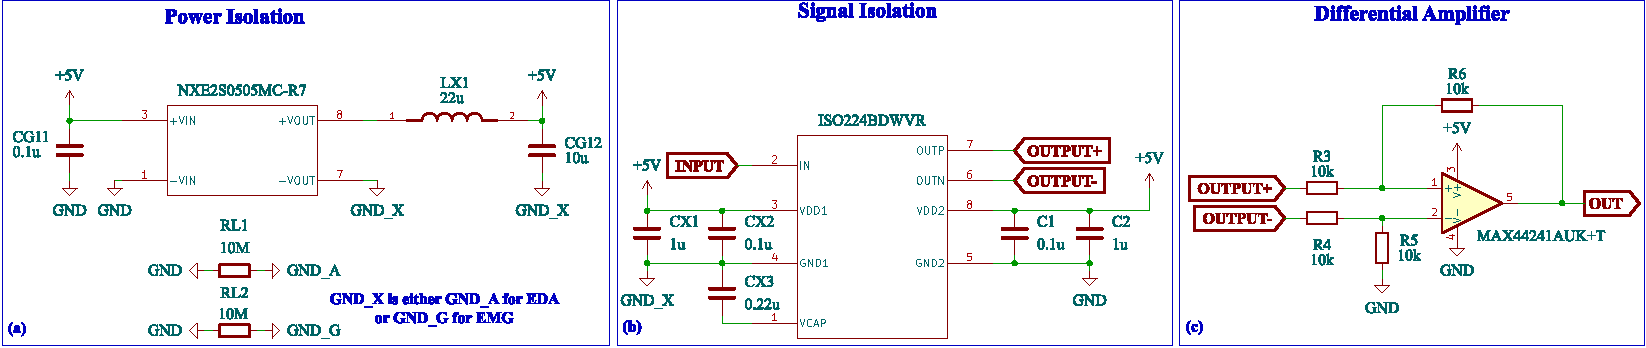
\includegraphics[width=\textwidth]{figures/version_2_figures-Galvanic Isolation (cropped) (pdfresizer.com).pdf}
    \caption{Building blocks of galvanic isolation. \textbf{(a)} Power isolation. \textbf{(b)} Signal isolation. \textbf{(c)} Differential amplifier.}
    \label{fig:isolation_blocks}
\end{figure}

\subsubsection{Architecture of Ground Domains}

The isolation process created three distinct ground domains, as represented in Fig.~\ref{fig:system_architecture}: GND for the power supply unit (PSU) and data acquisition (DAQ) card, GND\_G for the EMG front-end, and GND\_A for the EDA front-end. Resistors \( R_{L1} = R_{L2} = \SI{10}{\mega\ohm} \) connected each isolated domain to GND to prevent floating of the isolated planes. The high resistance value ensured that minimal current flowed between the domains.

\subsubsection{Power Isolation}

Each front-end was powered by a dedicated NXE2S0505MC-R7 isolated DC-DC converter (\SI{5}{\volt} input, \SI{5}{\volt} output, \SI{2}{\watt}), as depicted in Fig.~\ref{fig:isolation_blocks}a. The output filter adhered to the recommended application circuit from the datasheet~\cite{noauthor_nxe2s0505mcisolated_nodate}, featuring a \SI{22}{\micro\henry} inductor and decoupling capacitors.

\subsubsection{Signal Isolation}

For signal isolation, the ISO224 reinforced-isolated amplifier was used, implemented according to the recommended application circuit in the datasheet~\cite{noauthor_iso224_nodate}, as shown in Fig.~\ref{fig:isolation_blocks}b. Both front-ends operated from a \SI{5}{\volt} supply, ensuring that all signals remained well within the ISO224's allowable input range of \SI{\pm 12}{\volt}. The ISO224 had a fixed gain of \(1/3\), determined by component availability rather than by a specific design target. On the non-isolated side, the output was differential with a common-mode voltage of \( V_{DD2}/2 = \SI{2.5}{\volt} \). A unity-gain differential amplifier (MAX44241AUK+T, using four matched \SI{10}{\kilo\ohm} resistors) converted this to a single-ended signal, effectively canceling the \SI{2.5}{\volt} offset, as illustrated in Fig.~\ref{fig:isolation_blocks}c.

After isolation, the expected signal levels were approximately \SI{0.6}{\volt} peak with a \SI{0.41}{\volt} DC offset for EMG signals, and approximately \SI{0.8}{\volt} for EDA signals. The DAQ input range was configured to \SI{\pm 5}{\volt}, chosen to provide sufficient headroom for the anticipated signals while optimizing ADC resolution. The validation of the isolated system is addressed in Section~\ref{sec:validation}.


\subsection{Power Supply}
\label{sec:PSU}
The circuit operates from a USB-C power supply, which provides \SI{5}{\volt} on the non-isolated ground (GND) domain. Each front-end derives its own isolated rail from this supply using the NXE2S0505MC-R7 DC-DC converters, as described in Section~\ref{sec:galvanic_isolation}. The data acquisition (DAQ) card is powered independently from the mains, with no shared power path with the circuit. The various power supply building blocks are illustrated in Fig.~\ref{fig:power_blocks}.

\begin{figure}[H]
    \centering
    \begin{minipage}[t]{0.45\textwidth}
        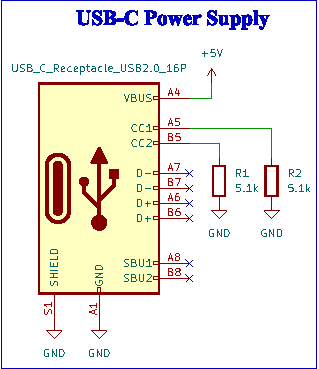
\includegraphics[height=0.28\textheight, keepaspectratio] {figures/version_2_figures-USB-C (cropped) (pdfresizer.com).pdf}
        \subcaption{USB-C power supply.}
        \label{fig:power_usbc}
    \end{minipage}
    \hfill
    \begin{minipage}[t]{0.45\textwidth}
        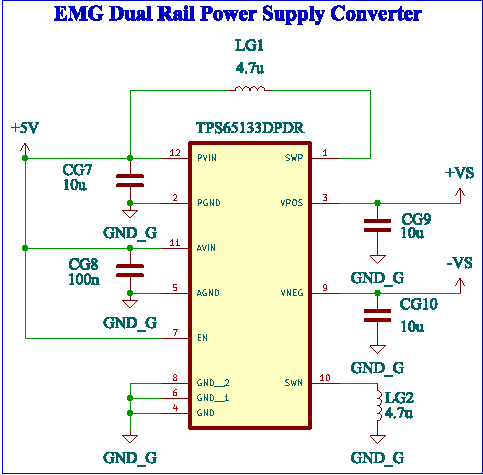
\includegraphics[height=0.28\textheight, keepaspectratio] {figures/version_2_figures-EMG Power Supply (cropped) (pdfresizer.com).pdf}
        \subcaption{EMG dual-rail power supply.}
        \label{fig:power_emg}
    \end{minipage}
    \vspace{1em}
    \begin{minipage}[t]{0.45\textwidth}
        \centering
        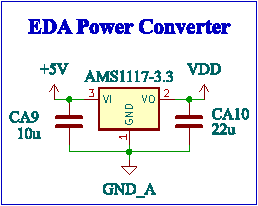
\includegraphics[width=\textwidth]{figures/version_2_figures-EDA Power Converter (cropped) (pdfresizer.com).pdf}
        \subcaption{EDA power converter.}
        \label{fig:power_eda}
    \end{minipage}
    \caption{Power supply building blocks. 
    \textbf{(a)} USB-C receptacle providing the \SI{5}{\volt} system supply via VBUS. 
    \textbf{(b)} TPS65133 dual-rail converter generating \SI{\pm 5}{\volt} for the EMG front-end on the GND\_G domain. 
    \textbf{(c)} AMS1117-3.3 linear regulator generating \SI{3.3}{\volt} for the EDA front-end on the GND\_A domain.}
    \label{fig:power_blocks}
\end{figure}

\subsubsection{USB-C Power Supply}
The \SI{5}{\volt} rail is derived from the VBUS pin of a USB-C receptacle, as depicted in Fig.~\ref{fig:power_blocks}a. Two \SI{5.1}{\kilo\ohm} pull-down resistors on CC1 and CC2 identify the circuit as a power sink to the host, prompting it to supply \SI{5}{\volt} without requiring active power delivery negotiation~\cite{noauthor_usb_nodate}. The data lines and sideband use (SBU) pins are left unconnected, as the connector is solely utilized for power.

\subsubsection{EMG Power Supply}
\label{sec:EMG_power}
The EMG front-end necessitates a dual-rail supply for the INA828 and signal-conditioning operational amplifiers (op-amps). A TPS65133DPDR generates \SI{\pm 5}{\volt} from the isolated \SI{5}{\volt} input on GND\_G, as illustrated in Fig.~\ref{fig:power_blocks}b. The output filter adheres to the recommended application circuit from the datasheet~\cite{noauthor_tps65133_nodate}, with $L_{G1} = L_{G2} = \SI{4.7}{\micro\henry}$ and decoupling capacitors on both rails.

\subsubsection{EDA Power Supply}
\label{sec:EDA_power}
The EDA front-end operates on a single \SI{3.3}{\volt} rail. An AMS1117-3.3 regulator converts the isolated \SI{5}{\volt} from GND\_A to \SI{3.3}{\volt}, as shown in Fig.~\ref{fig:power_blocks}c. An input capacitor $C_{A9} = \SI{10}{\micro\farad}$ and an output capacitor $C_{A10} = \SI{22}{\micro\farad}$ follow the recommended application circuit from the datasheet~\cite{evvo_ams1117_nodate}. This rail serves as VDD for both the current source and the virtual ground divider in the EDA front-end.

The equipment and software used to validate this hardware are described in the following section.


\section{Equipment, Materials, and Software tools}
Physical equipment used in the validation protocol is listed in Table~\ref{tab:validation_equipment}. Table~\ref{tab:hardware_tools} describes the custom hardware developed for this thesis, and Table~\ref{tab:software_tools} lists the software tools used for design, acquisition, and analysis.

\begin{table}[H]
\centering
\caption{Custom hardware.}
\label{tab:hardware_tools}
\begin{tabularx}{\textwidth}{l l X}
\toprule
\textbf{Item} & \textbf{Specification} & \textbf{Notes} \\
\midrule
Custom analog front-end & EMG/EDA acquisition circuit &
    \parbox[t]{\linewidth}{\small
        - Custom PCB \\
        - Powered via USB-C \\
        - See Sec.~\ref{sec:system_architecture}} \\
\bottomrule
\end{tabularx}
\end{table}

\begin{table}[H]
\centering
\caption{Software tools.}
\label{tab:software_tools}
\begin{tabularx}{\textwidth}{p{5.5cm} l X}
\toprule
\textbf{Tool} & \textbf{Version} & \textbf{Purpose} \\
\midrule
KiCad & 9.0.6 & Schematic capture and PCB layout \\
\addlinespace
LTspice & 26.0.1 & Circuit simulation and frequency response \\
\addlinespace
NI-DAQmx & 2025 Q3 & Hardware driver for NI USB-6356 \\
\addlinespace
Python & 3.10.4 & Acquisition and analysis \\
\addlinespace
\quad\texttt{numpy}      & --- & Numerical computation \\
\quad\texttt{scipy}      & --- & Signal processing \\
\quad\texttt{matplotlib} & --- & Plotting \\
\quad\texttt{pandas}     & --- & Data handling \\
\quad\texttt{nidaqmx}    & --- & NI hardware interface \\
\quad\texttt{nptdms}     & --- & TDMS file read and write \\
\quad\texttt{PyQt6}      & --- & GUI framework \\
\quad\texttt{pyqtgraph}  & --- & Real-time signal plotting \\
\addlinespace
VS Code / Jupyter & --- & Development environment \\
\addlinespace
\texttt{daq\_gui\_multi\_validation.py} & --- &
    Custom real-time acquisition GUI \\
\texttt{analysis\_utils.py} & --- &
    Custom offline analysis library \\
\texttt{validation\_analysis.ipynb} & --- &
    Analysis notebook for (Q1-Q7) \\
\bottomrule
\end{tabularx}
\end{table}

The validation protocol that used this equipment is described in the following section.

\section{Validation Protocol}
\label{sec:validation}


%\subsection{Aim}
%To validate a custom circuit for simultaneous measurement of surface EMG and EDA from the same muscle area. Validation proceeds in two stages: individual circuit verification (Sessions 1 and 2), followed by simultaneous measurement validation (Sessions 3--5).

\subsection{Validation Questions}
\label{sec:validation_Q}
\begin{enumerate}
    \item How does the galvanic isolation stage affect signal amplitude and frequency content?
    \item What are the signal characteristics of the EMG front-end during isolated muscle contraction, and what are its limitations?
    \item What are the signal characteristics of the EDA front-end during isolated measurement, and what are its limitations?
    \item How does digital post-filtering affect EMG signal quality at the pre- and post-isolation stages?%EMG signal only
    \item How does simultaneous EMG acquisition affect the EDA measurement?
    \item How does simultaneous EDA acquisition affect the EMG measurement?
    \item How consistent are the EMG and EDA measurements across repeated simultaneous recording sessions?
\end{enumerate}

\subsection{Participants}
One healthy adult (the author), right-handed, with no known neuromuscular or dermatological disorders affecting the hands. This is a technical self-experiment conducted solely for circuit validation.

\subsection{Equipment and Setup}

\begin{table}[H]
\centering
\caption{Equipment used in the validation protocol.}
\label{tab:validation_equipment}
\begin{tabular}{l l p{4.5cm}}
\toprule
\textbf{Item} & \textbf{Model / Specification} & \textbf{Notes} \\
\midrule
Custom circuit & EMG/EDA front-end & See Fig.~\ref{fig:system_architecture} \\
\addlinespace
Electrodes & Kendall H135SG & \parbox[t]{4.5cm}{\small - Type: H135SG, \newline Ref: 31.1355.21 \newline - Material: Ag/AgCl \newline - Size: 43$\times$35~mm \newline - Disposable, pre-gelled} \\
\addlinespace
DAQ card & NI USB-6356 & \parbox[t]{4.5cm}{\small - $f_s = 2000$~Hz, all channels \newline - Input range: $\pm\SI{2}{\volt}$ \newline - Resolution: 16-bit \newline  - Input configuration: Floating Source (FS) \newline - Python 3.10.4, \texttt{nidaqmx}} \\

\addlinespace
Multimeter & UNI-T UT131B & Resistance mode for FSR \\
\addlinespace
Force sensor & Interlink Electronics FSR400 & \SI{200}{\ohm}-\SI{100}{\kilo\ohm} \\
\addlinespace
Environment & Quiet room, 21-24~$^\circ$C & Recordings 09:00-12:00 \\
\bottomrule
\end{tabular}
\end{table}

\subsection{Acquisition Software}
\label{sec:acquisition_software}
A custom Python script, \texttt{daq\_gui\_multi\_validation.py},  handled data acquisition throughout all sessions. It interfaced with the NI USB-6356 via the \texttt{nidaqmx} library and sampled all active channels simultaneously at \SI{2}{\kilo\hertz}. Raw data were written to disk in TDMS format throughout each session. A real-time digital filter chain ran in parallel for visual monitoring and was excluded from the offline analysis. Stimulus cues were delivered through the graphical interface, and their onset timestamps were saved as event markers in the TDMS file for epoch extraction during post-processing.

\subsection{Electrode Placement and Skin Preparation}

\subsubsection{Skin Preparation}
The participant washed both hands with soap and water and dried them thoroughly with a paper towel. No lotion, cream, or skin products were applied to the hands or wrists on the morning of the recording. Jewelry was removed from the left hand and wrist.

\subsubsection{Electrode Placement}
The target recording site for clinical deployment is the biceps, where EMG and EDA electrodes are co-located on the same muscle. For this technical validation, the hand was used instead. Palmar EDA is the established measurement site in the literature, and thenar EMG is well-characterized, so the hand provided a known reference against which circuit performance could be benchmarked before moving to the biceps site. 
Electrode positions are shown in Figure~\ref{fig:hand_electrode_placement}.

\begin{figure}[H]
    \centering
    \colorbox{white}{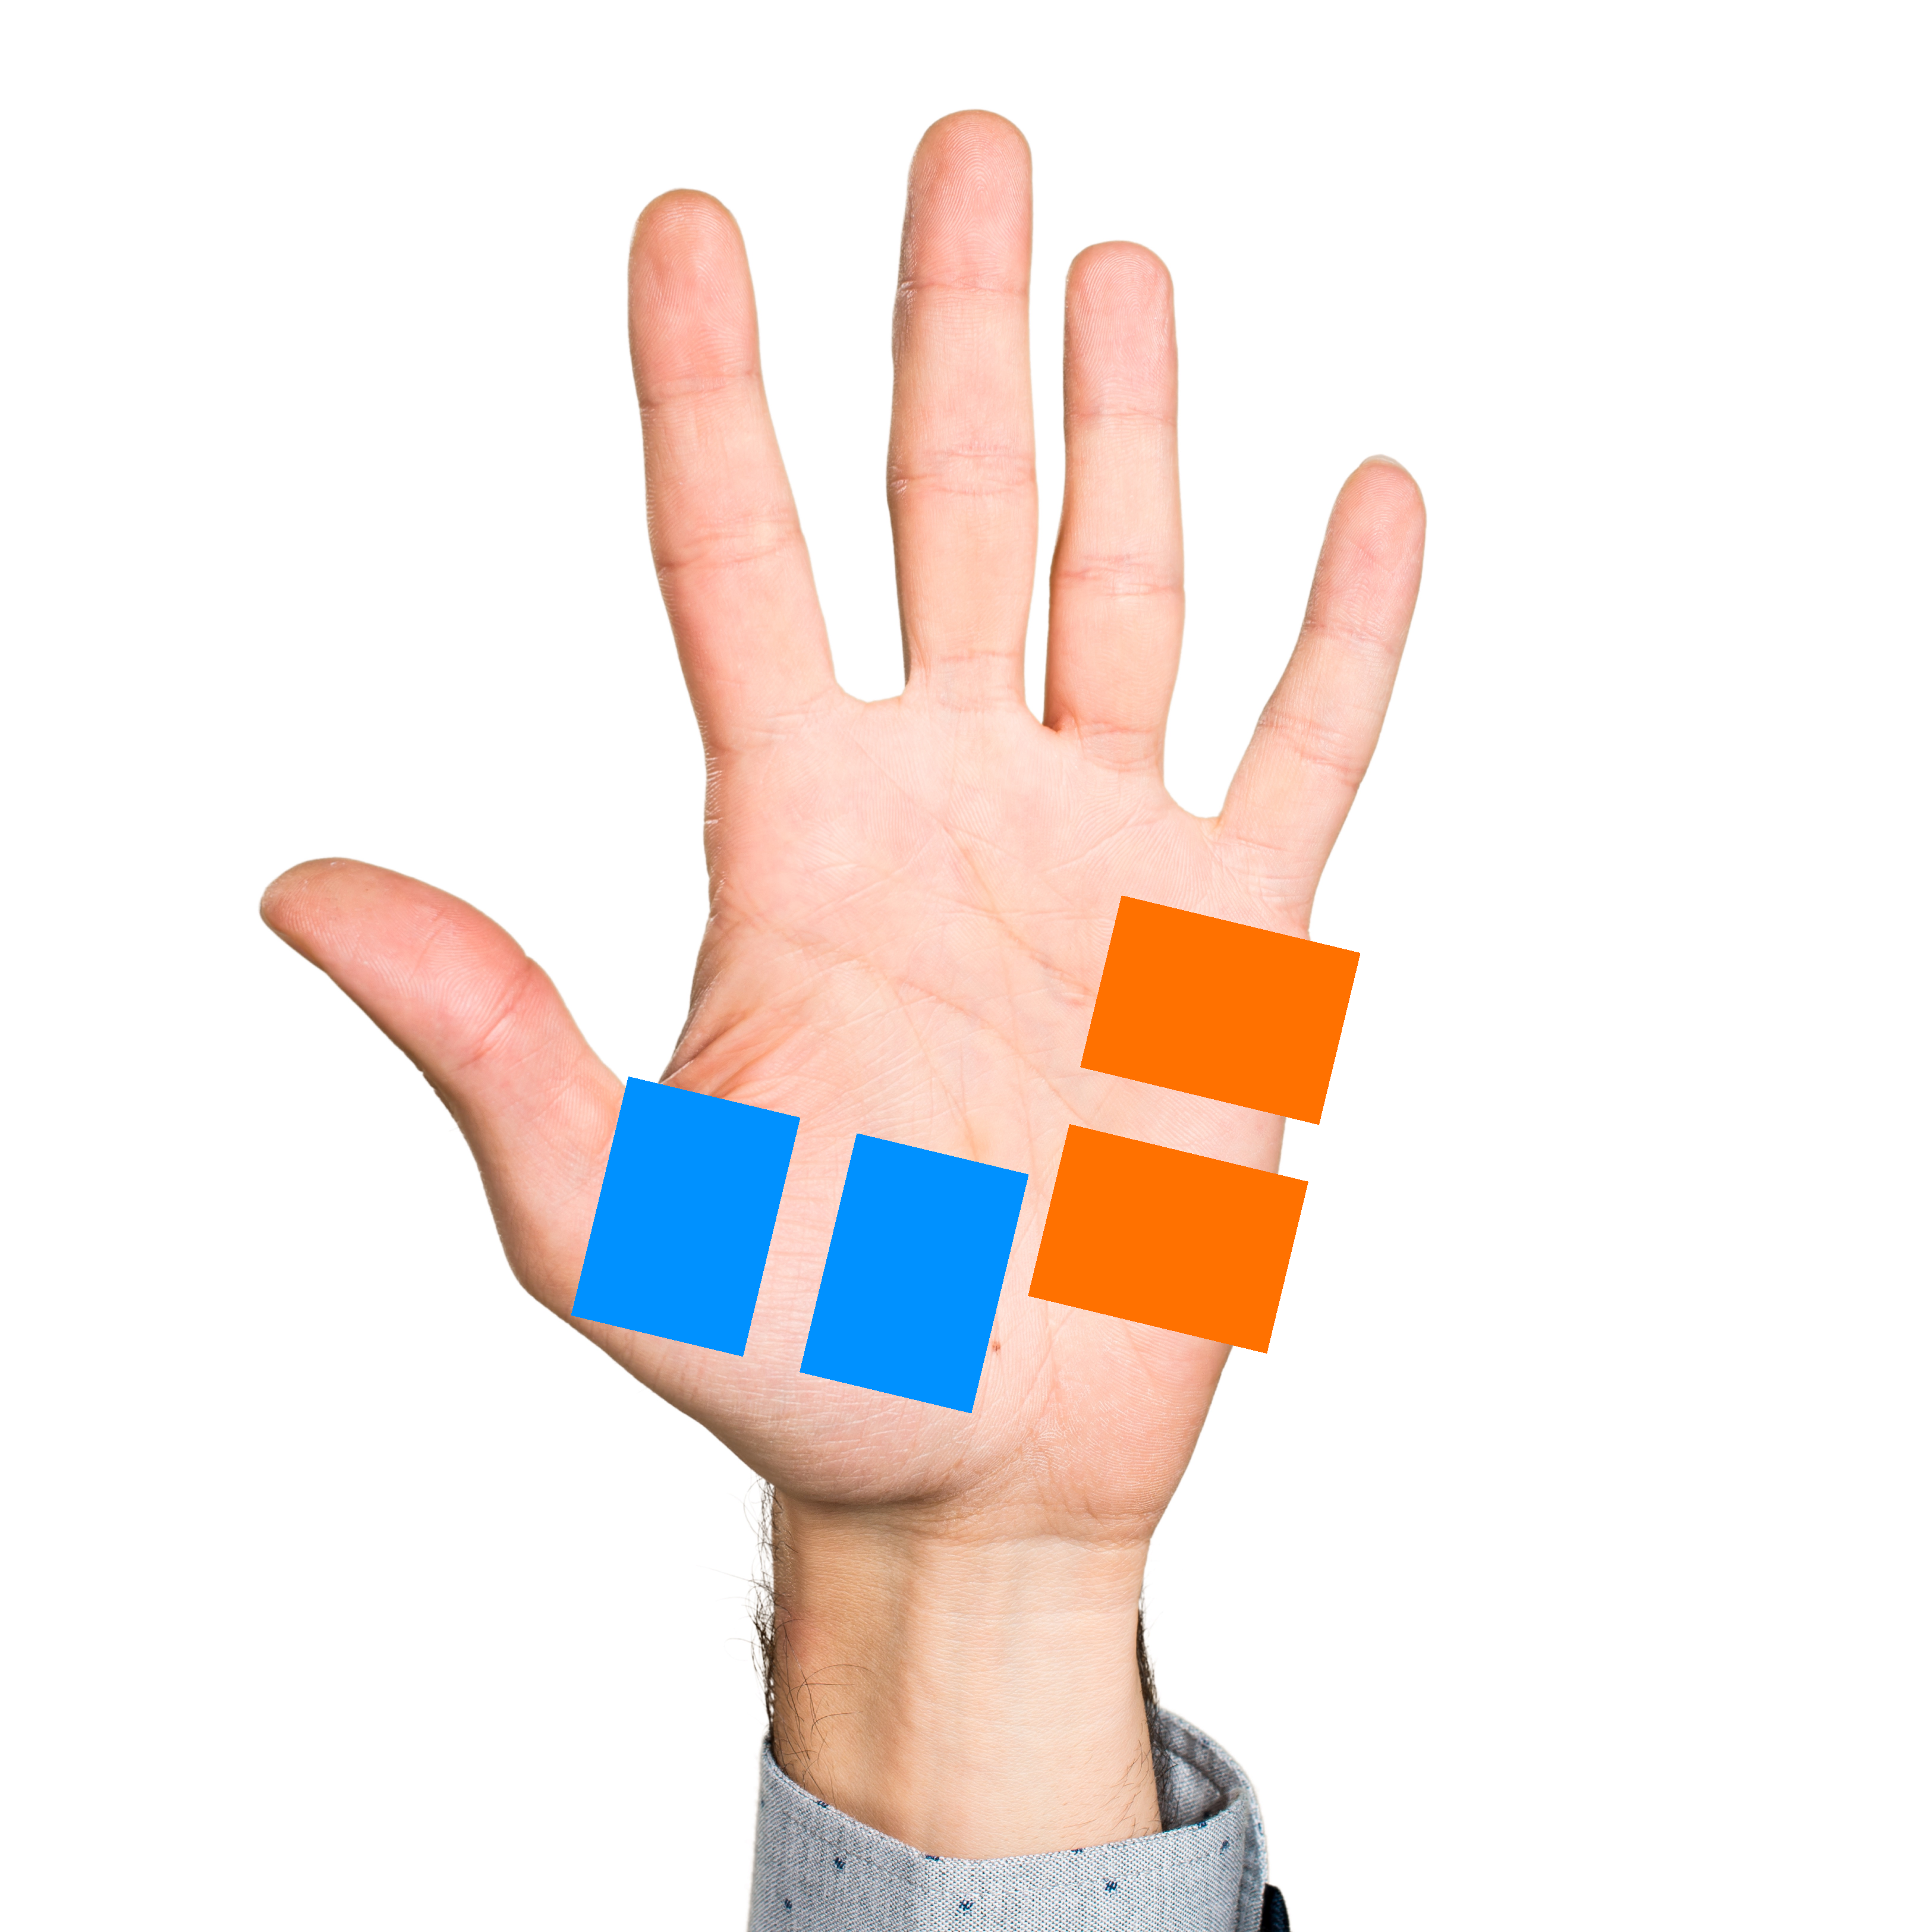
\includegraphics[width=0.5\linewidth]{figures/hand_electrode_placement (converted) (pdfresizer.com).pdf}}
    \caption{Electrode placement on the palmar surface of the left hand. Blue: EMG 
    recording electrodes over the thenar eminence. Orange: EDA electrodes over the 
    hypothenar eminence.}
    \label{fig:hand_electrode_placement}
\end{figure}

Three electrodes were used for EMG and two for EDA (Figure is coming later). For EMG, two recording electrodes were placed over the thenar eminence of the left hand in a bipolar configuration, aligned approximately along the proximal-distal axis of the thumb musculature with an inter-electrode distance of 10~mm (edge-to-edge). The EMG reference electrode was placed on the dorsal aspect of the left forearm, approximately 5~cm distal to the elbow. For EDA, two electrodes were placed on the palmar surface over the hypothenar eminence of the left hand, with a center-to-center distance of approximately 10~mm.


%Revised version
\begin{comment}
Three electrode configurations are tested across sessions:

\textbf{Configuration A (original):} Two EMG recording electrodes over the
thenar eminence in bipolar configuration, aligned along the proximal--distal
axis with 10\,mm edge-to-edge separation. Two EDA electrodes over the
lumbrical region between the index and middle fingers.

\textbf{Configuration B (supervisor suggestion, left):} One EMG electrode
placed over the muscle belly (largest thenar mass) and one more distally on
the proximal thumb phalanx, mimicking a clinical CMAP recording arrangement.
Two EDA electrodes placed over the hypothenar eminence (a well-established
EDA measurement site. This configuration maximizes expected EMG amplitude
and spatially separates EMG and EDA electrode fields.

\textbf{Configuration C (supervisor suggestion, right):} EMG electrodes
positioned within the current path between the two EDA electrodes, to
stress-test whether cross-interference occurs under the worst-case spatial
overlap.
\end{comment}

\subsection{Outcome Measures and Success Criteria}

\begin{itemize}
    \item Signal quality
    \item Minimal interference
    \item Reproducibility
\end{itemize}

(Discuss with supervisors what requirements to have)

\subsection{Stimulation Instructions}

%Stimulation cue onset timestamps were saved as event markers in the TDMS file during acquisition.
\paragraph{EMG Stimulation}
The participant sat with the left forearm resting on the table, elbow flexed approximately 90$^\circ$ and the palm facing up. The fingers were relaxed in a neutral, slightly open position. 

An FSR400 force sensor was placed on top of the index finger before each block and remained in position throughout. At each EMG stimulus cue, the participant brought the thumb tip into contact with the index finger tip as quickly as possible and held the contraction for \SI{1}{\second}. A multimeter connected to the FSR400 provided real-time resistance feedback, and the participant adjusted force to maintain the sensor resistance at approximately \SI{5}{\kilo\ohm} during each contraction. Based on the FSR400 datasheet~\cite{inc_fsr_nodate}, \SI{5}{\kilo\ohm} corresponds to approximately 100~gf. After \SI{1}{\second}, the participant relaxed the hand and returned to the neutral position.

\paragraph{EDA Stimulation}
At each EDA stimulus cue, the participant inhaled deeply over 2~seconds from normal breathing, then exhaled normally and relaxed. A visual or auditory cue from the control software guided the timing of the deep breath.

\subsection{Recording Procedure}

All sessions followed the same structure: 10~minutes of baseline recording followed by a 30-minute test run. Sessions 1 and 2 verified each circuit individually, with only one circuit connected at a time. Sessions 3-5 validated simultaneous operation with both circuits connected.

\subsubsection{Session 1: EMG Circuit Verification}
Only the EMG circuit was connected. The EDA circuit was physically disconnected. Two channels were recorded simultaneously throughout:
\begin{itemize}
    \item Pre-isolation, unfiltered (raw)
    \item Post-isolation, unfiltered (raw)
\end{itemize}

\begin{enumerate}
    \item Electrodes were applied as described above (EMG electrodes only).
    \item The participant rested quietly for 30~minutes to allow the electrode-skin impedance to stabilize.
    \item During the final 10~minutes of this period, baseline EMG was recorded on both channels
    \item The 30-minute test run began. Every 15~seconds, a cue prompted the participant to perform one EMG stimulus for 2~seconds, followed by relaxation. This yielded 120 EMG stimuli.
\end{enumerate}

Post-session analysis of Session~1 data is described in Sections~\ref{sec:emg_processing} and~\ref{sec:comparative_analysis}.

\subsubsection{Session 2: EDA Circuit Verification}
Only the EDA circuit was connected. The EMG circuit was physically disconnected. Two channels were recorded simultaneously throughout: pre-isolation raw and post-isolation raw.

\begin{enumerate}
    \item Electrodes were applied as described above (EDA electrodes only).
    \item The participant rested quietly for 30~minutes to allow the electrode-skin impedance to stabilize.
    \item During the final 10~minutes of this period, baseline EDA was recorded on both channels. The post-isolation baseline served as the session-level EDA noise floor in the analysis described in Section~\ref{sec:eda_processing}.
    \item The 30-minute test run began. Every 60~seconds, a cue prompted the participant to perform one deep-breath EDA stimulus. This yielded 30 EDA stimuli.
\end{enumerate}

Post-session analysis of Session~2 data is described in Sections~\ref{sec:eda_processing} and~\ref{sec:comparative_analysis}.

\subsubsection{Sessions 3-5: Simultaneous EMG and EDA}
Both circuits were connected simultaneously. Each session consisted of 10~minutes of baseline recording followed by three consecutive 10-minute blocks.

\begin{enumerate}
    \item EMG and EDA electrodes were applied as described above.
    \item The participant rested quietly for 30 minutes to allow the electrode-skin impedance to stabilize.
    \item During the final 10~minutes of this period, baseline EMG and EDA signals were recorded while the participant remained still and breathed normally. The post-isolation EDA baseline served as the session-level EDA noise floor in the analysis described in Section~\ref{sec:eda_processing}.
    \item The 30-minute test run consisted of three 10-minute blocks:
    \begin{enumerate}
        \item \textbf{Block 1: EDA-only (10 minutes)}\\ The participant remained seated with the left hand resting in the neutral position. Every 60 seconds, a cue prompted one deep-breath EDA stimulus. No voluntary hand or finger movement was performed. This block yielded 10 EDA stimuli.
        \item \textbf{Block 2: EMG-only (10 minutes)}\\ Every 15~seconds, a cue prompted one EMG stimulus for 2~seconds, followed by relaxation. No deep-breath EDA stimuli were performed. This block yielded 40 EMG stimuli.
        \item \textbf{Block 3: Combined EMG and EDA (10 minutes)}\\ Both stimulus types were performed according to the same timing as Blocks 1 and 2. The EDA cue fired first; the EMG cue was delayed by \SI{5}{\second} relative to the EDA cue. This block yielded 10 EDA stimuli and 40 EMG stimuli.
    \end{enumerate}
    \item In total, one session yielded 20 EDA stimuli (10 in EDA-only + 10 in combined) and 80 EMG stimuli (40 in EMG-only + 40 in combined).
    \item Sessions 3-5 were conducted on three separate days under the same conditions.
    \item The block order was fixed across Sessions~3-5: EDA-Only first, EMG-Only second, and Combined last. This fixed order means that time-on-task effects, such as habituation in EDA or fatigue in EMG, cannot be separated from block-specific effects in the analysis.
\end{enumerate}


\section{Signal Processing and Data Analysis}
%Full validation chain is: isolation works (Q3) → each signal is clean in isolation (Q1/Q2) → simultaneous operation doesn't degrade either signal (Q5/Q6).
%In short, RMS is appropriate when the mean is zero. std is appropriate when the mean carries information you want to preserve.
EMG and EDA signals were processed through separate pipelines, each matched to the physical nature of the signal. Both pipelines operated on raw TDMS recordings and produced the metrics used to answer Q1 to Q7, as illustrated in Figure~\ref{fig:data_analysis_pipeline}. Gain compensation is described in Section~\ref{sec:gain_compensation}, core analysis methods in Section~\ref{sec:core_analysis}, and signal-specific processing in Sections~\ref{sec:emg_processing} and~\ref{sec:eda_processing}. The comparative analysis is covered in Section~\ref{sec:comparative_analysis}.

\begin{figure}[H]
    \centering
    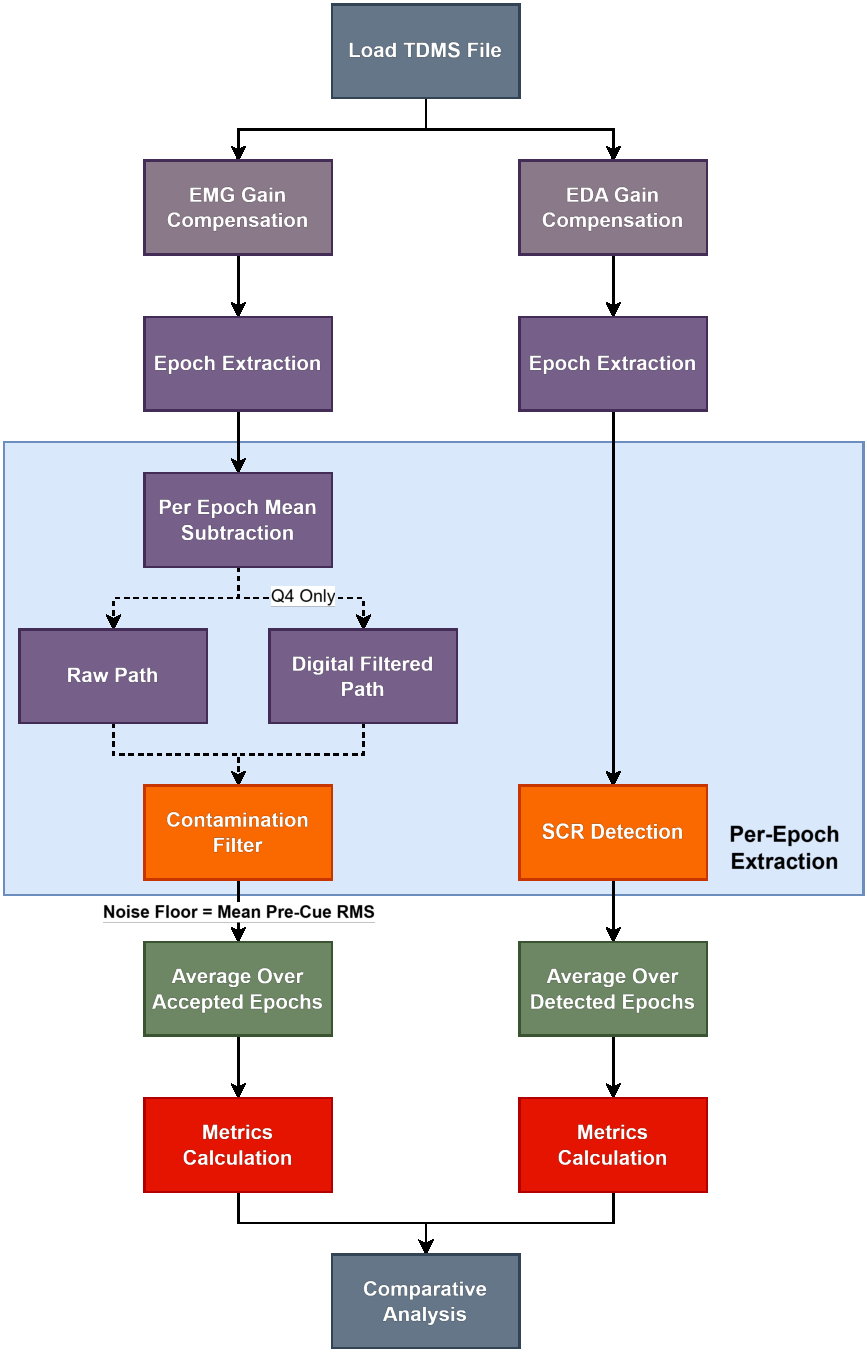
\includegraphics[height=\textheight]{figures/Data_analysis_pipeline.drawio (converted) (pdfresizer.com).pdf}
    \caption{A high-level view of the data processing pipeline. All metric computations are grouped into a single 'Metrics Calculation' block. Full metric definitions are given in Sections~\ref{sec:emg_processing} and~\ref{sec:eda_processing}.}
    \label{fig:data_analysis_pipeline}
\end{figure}

\subsection{Gain Compensation}\label{sec:gain_compensation}
Both front-ends introduce gain that must be removed before computing any metrics. Gain compensation was applied once at data load, converting all channels to physical units (\si{\micro\volt} for EMG, \si{\micro\siemens} for EDA). The compensation steps for each channel type are listed in Table~\ref{tab:gain_compensation}. The EMG chain gain of \num{733.3} is derived in Section~\ref{sec:EMG_total_gain}. For EDA, the $\times 2$ low-pass filter gain is absorbed into Equation~\ref{eq:EDA_skin_resistance}, so no additional correction is needed beyond the $\times 3$ ISO224 factor for post-isolation channels, as described in Section~\ref{sec:EDA_frontend}. 

\begin{table}[H]
\centering
\caption{Load-time gain compensation applied to each channel type.}
\label{tab:gain_compensation}
\begin{tabularx}{\textwidth}{l l l X}
\toprule
\textbf{Channel} & \textbf{Isolation} & \textbf{Operation} & \textbf{Output} \\
\midrule
EMG & Pre  & $\div 733.3$                        & \si{\micro\volt} \\
\addlinespace
EMG & Post & $\times 3 \div 733.3$               & \si{\micro\volt} \\
\addlinespace
EDA & Pre  & Eq.~\ref{eq:EDA_skin_resistance}, inverted       & \si{\micro\siemens} \\
\addlinespace
EDA & Post & $\times 3$, then Eq.~\ref{eq:EDA_skin_resistance}, inverted & \si{\micro\siemens} \\
\bottomrule
\end{tabularx}
\end{table}


\subsection{Core Analysis Methods}
\label{sec:core_analysis}
%Four methods used: RMS, SNR, attenuation, PSD - signal-agnostic definitions only

Five methods were used throughout this work to answer Q1-Q7 (Section~\ref{sec:validation_Q}): Root Mean Square (RMS), Signal-to-Noise Ratio (SNR), attenuation, Power Spectral Density (PSD), and Pearson correlation. Each is defined here in signal-agnostic terms. Signal-specific implementations are given in Sections~\ref{sec:emg_processing} and~\ref{sec:eda_processing}.

%RMS definition and equation - EMG only, state this explicitly, why not EDA
RMS measured signal power over a fixed time window. For a discrete signal $x[n]$ over $N$ samples, RMS is defined as
\begin{equation}
    \text{RMS} = \sqrt{\frac{1}{N}\sum_{n=1}^{N} x[n]^2}
    \label{eq:rms}
\end{equation}
RMS was applied only to the EMG signal. For EMG, the arithmetic mean is uninformative because the signal oscillates symmetrically around zero; squaring each sample before averaging removes this problem and gives a direct measure of signal amplitude. RMS was not applied to EDA. The DC-coupled EDA signal has a large non-zero mean from the tonic skin conductance level, so an RMS computed over EDA reflects that mean rather than the noise floor and carries no useful noise information. RMS is the standard amplitude measure in surface EMG literature~\cite{kamen_essentials_2010}.

%SNR - general equation, S and N deferred
SNR expressed the amplitude of a desired signal relative to background noise:
\begin{equation}
    \text{SNR}_\text{dB} = 20\log_{10}\left(\frac{S}{N}\right)
    \label{eq:snr}
\end{equation}
where $S$ is the signal amplitude and $N$ is the noise floor. The definitions of $S$ and $N$ differ between EMG and EDA and are given in Sections~\ref{sec:emg_processing} and~\ref{sec:eda_processing}.

%Attenuation - generic X, defined per signal downstream, used in Q1
Attenuation quantified how well the isolation stage preserved signal amplitude after compensating for the fixed gain of $\nicefrac{1}{3}$ introduced by the ISO224 (Section~\ref{sec:galvanic_isolation}). A value of \SI{0}{\decibel} indicated perfect amplitude preservation:
\begin{equation}
    A_\text{dB} = 20\log_{10}\left(\frac{X_\text{post}}{X_\text{pre}}\right)
    \label{eq:attenuation}
\end{equation}
where $X$ is an amplitude measure defined per signal in Sections~\ref{sec:emg_processing} and~\ref{sec:eda_processing}.

%PSD - Welch's method, purpose only, parameters in signal-specific sections
PSD was estimated using Welch's method, which averaged periodograms of overlapping signal segments to reduce spectral variance. The PSD verified that signal energy remained within the expected frequency band and identified spectral interference from simultaneous circuit operation. The following two sections describe how each method was applied to the EMG and EDA signals, respectively.

%Pearson correlation - morphology preservation, used in Q1
Pearson correlation quantified the linear similarity between two signals. For two discrete signals $x[n]$ and $y[n]$ of length $N$, the Pearson correlation coefficient is defined as
\begin{equation}
    r = \frac{\sum_{n=1}^{N}\left(x[n] - \bar{x}\right)\left(y[n] - \bar{y}\right)}{\sqrt{\sum_{n=1}^{N}\left(x[n] - \bar{x}\right)^2}\,\sqrt{\sum_{n=1}^{N}\left(y[n] - \bar{y}\right)^2}}
    \label{eq:pearson}
\end{equation}
where $\bar{x}$ and $\bar{y}$ are the sample means. The coefficient ranges from $-1$ to $+1$. A value of $+1$ indicates an identical waveform shape. Pearson correlation was used in Q1 to verify that the isolation stage preserved signal morphology. The following two sections describe how each method was applied to the EMG and EDA signals, respectively.

%A session-wide RMS would collapse the entire recording to a single power estimate and lose temporal resolution. Moving the window sample by sample yielded one RMS value per sample, preserving the time course of muscle activity.

%EMG is bipolar, so the signal was rectified before the window was applied. Without rectification, positive and negative values would partially cancel within each window, underestimating the true signal amplitude.
\subsection{EMG Signal Processing}
\label{sec:emg_processing}
%Pipeline order: epoch extraction → mean subtraction → scalar RMS → Q4 branch → contamination filter → noise floor → sliding window RMS → S and N definitions → PSD parameters

The following section describes, in pipeline order, how the core analysis methods were applied to the EMG signal.

%Epoch extraction (-0.5 to +3.5s), contraction window (0-1.2s), pre-cue (-0.5 to 0s), recovery for visualisation
The continuous EMG recording was segmented into epochs time-locked to each contraction cue. Each epoch spanned from \SI{0.5}{\second} before to \SI{3.5}{\second} after the cue onset, giving a \SI{4}{\second} window per contraction. Cue onset timestamps were extracted from the event markers stored in the TDMS file during acquisition. Two sub-windows were defined within each epoch: the pre-cue window from \SIrange{-0.5}{0}{\second} relative to the cue for DC offset estimation and noise floor computation, and the contraction window from \SIrange{0.0}{1.2}{\second} for signal amplitude estimation. The contraction window was shorter than the expected contraction duration to ensure it fell fully within the active contraction period, regardless of trial-to-trial variation in contraction length. A recovery period from \SIrange{1.2}{3.5}{\second} was retained for visualization only.

%Per-epoch mean subtraction - pre-cue mean, not full epoch, reason
After extraction, the DC offset was removed from each epoch individually. The mean of the pre-cue window was computed and subtracted from all samples in that epoch. Using the pre-cue window rather than the full epoch mean avoided bias from the contraction, which would otherwise elevate the epoch mean and suppress both the baseline and contraction estimates. This step removed static DC contributions from the voltage lifting circuit (Section~\ref{sec:EMG_frontend}), electrode half-cell potentials, and amplifier input offsets.

%Scalar RMS - two values per epoch
Two scalar RMS values were computed per epoch using Equation~\ref{eq:rms}. The pre-cue RMS was calculated across all samples within the pre-cue window and served as the per-epoch noise-floor estimate. The contraction RMS was calculated over all samples in the contraction window and served as the signal amplitude estimate.

%Q4 parallel path - filter chain after mean subtraction, zero-phase, notch BW
To address Q4, a three-stage digital filter chain was applied offline after mean subtraction, creating a parallel path alongside the unfiltered signal. The chain consisted of a second-order Butterworth HPF at \SI{20}{\hertz}, an IIR notch at \SI{50}{\hertz} with $Q = 30$, and a fourth-order Butterworth LPF at \SI{500}{\hertz}. All stages used zero-phase filtering via \texttt{filtfilt}, which applied each filter in the forward and backward directions to eliminate phase distortion. Zero-phase filtering was not available in the real-time analog chain because it requires access to future samples. The digital notch bandwidth was
\begin{equation}
    \Delta f = \frac{f_0}{Q} = \frac{\SI{50}{\hertz}}{30} \approx \SI{1.67}{\hertz}
    \label{eq:digital_notch_bw}
\end{equation}
This was narrower than the analog twin-T notch bandwidth of \SI{10.5}{\hertz} ($Q \approx 5$, Equation~\ref{eq:notch_q}), preserving more EMG spectral content around \SI{50}{\hertz}. All subsequent processing steps were applied identically to both paths.

%Contamination filter - empirical threshold, no citation
A contamination filter was applied to exclude epochs with elevated baseline activity before metric computation. An epoch was rejected if its pre-cue RMS exceeded twice the median pre-cue RMS across all epochs in the session ($\text{RMS}_\text{pre} > 2 \times \tilde{\text{RMS}}_\text{pre}$). This threshold was chosen empirically; no standard criterion exists in the EMG literature for this type of rejection. Epochs above the threshold likely contained motion artifacts or other baseline interference that would corrupt both the noise floor and contraction RMS estimates.

%Noise floor - mean pre-cue RMS across clean epochs, why per-epoch
The noise floor was the mean pre-cue RMS across all epochs that passed the contamination filter. This per-epoch approach tracked signal conditions at each contraction rather than relying on a session-level baseline that would not capture short-term changes in electrode contact or ambient noise.

%Sliding window RMS - linear envelope, visualization only, clean epochs only
Linear envelope detection was used to visualize the time course of muscle activation~\cite{kamen_essentials_2010}. The rectified EMG signal was processed with a \SI{100}{\milli\second} sliding RMS window, producing a smooth amplitude envelope that tracked muscle activity over time~\cite{konrad_abc_2006}. The \SI{100}{\milli\second} window balanced temporal resolution against stability of estimates. The sliding-window RMS was applied only to clean epochs and was not used in any metric computation.

%S and N definitions for EMG SNR - computation moved to comparative analysis
For EMG, $S$ in Equation~\ref{eq:snr} was the mean contraction RMS across clean epochs, and $N$ was the noise floor as defined above.

%PSD parameters for EMG
The PSD was computed over the full EMG recording using a \SI{1}{\second} window with 50\% overlap, covering the frequency band from \SIrange{10}{500}{\hertz}.

%Mains harmonic power - quantify residual power-line interference
Mains harmonic power was computed to quantify residual power-line interference in the EMG signal. Three harmonics were evaluated: the \SI{50}{\hertz} fundamental, and the \SI{100}{\hertz} and \SI{150}{\hertz} harmonics. For each harmonic, the power was integrated across a band of $\pm\SI{1.67}{\hertz}$ around the center frequency, equal to the digital notch bandwidth defined in Equation~\ref{eq:digital_notch_bw}:
\begin{equation}
    P_\text{harmonic}(f_0) = \int_{f_0 - \Delta f}^{f_0 + \Delta f} \text{PSD}(f)\, df
     \label{eq:harmonic_power}
\end{equation}
where $f_0$ is the harmonic center frequency and $\Delta f = \SI{1.67}{\hertz}$. The total mains harmonic power was the sum across the three harmonics. A low total harmonic power would indicate that the EMG front-end effectively rejected power-line interference. Elevated power at \SI{100}{\hertz} or \SI{150}{\hertz} would indicate that harmonic content described in Section~\ref{sec:emg_noise} was not suppressed by the \SI{50}{\hertz} notch filter. The EDA signal required a different processing approach due to its DC-coupled nature and slower response dynamics, as described in the following section.


\subsection{EDA Signal Processing}
\label{sec:eda_processing}
%Pipeline order: epoch extraction → no filtering → no mean subtraction → SCL → noise floor → SCR detection → epoch averaging → SNR definition

The following section describes how the EDA signal was quantified. As described in Section~\ref{sec:EDA_signal}, the EDA signal consists of a tonic component, the skin conductance level (SCL), and a phasic component, the skin conductance response (SCR). The sampled voltage $V_\text{EDA}$ was converted to skin conductance using Equation~\ref{eq:EDA_skin_resistance}, with measurements expressed in \si{\micro\siemens}.

%Epoch extraction (-2 to +10s), baseline -2 to 0s, why 12s window
The EDA recording was segmented into epochs time-locked to each breath-holding cue, as illustrated in Figure~\ref{fig:eda_epoch}A. Each epoch spanned from \SI{2}{\second} before to \SI{10}{\second} after the cue onset, giving a \SI{12}{\second} window per trial. The pre-cue segment from \SIrange{-2}{0}{\second} served as the per-epoch baseline for SCL and noise floor estimation. A longer pre-cue window than in the EMG case was used because EDA exhibits slower drift and requires more samples to obtain a stable tonic estimate. The post-cue window extended to \SI{10}{\second} to capture the full SCR morphology, including the recovery phase, which typically lasts several seconds after the response peak.

%No digital filtering + reason
No digital filtering was applied to the EDA signal. The \SI{1.5}{\hertz} analog low-pass filter in the EDA front-end (Section~\ref{sec:EDA_frontend}) already bandlimits the signal to the relevant EDA frequency range. Additional digital filtering risked distorting the slow SCR waveform dynamics that carried the physiological information of interest.

%No mean subtraction + reason
Mean subtraction was not applied to the EDA signal. Unlike EMG, EDA is DC-coupled, and its mean reflects the tonic skin conductance level. Removing the epoch mean would discard the SCL, which was itself a metric of interest.

%SCL - per-epoch pre-cue mean, why per-epoch, use in Q5
The SCL was computed as the mean conductance over the per-epoch pre-cue window, shown as the grey region in Figure~\ref{fig:eda_epoch}B. This operationalization differs from the conventional session-level SCL estimate~\cite{boucsein_electrodermal_2012} and was chosen to provide a tonic estimate representative of signal conditions at the time of each stimulus, while capturing habituation-driven drift across the recording. The SCL also served as a between-condition comparator in Q5 to detect tonic contamination from simultaneous EMG operation.

%Noise floor - two estimates, session-level circuit + per-epoch local, why not RMS
Two noise floor estimates were used for the EDA signal. The first was a session-level estimate computed from the \SI{10}{\minute} stabilization recording at the start of each session, during which the subject sat still with no stimulus. The recording was linearly detrended to remove residual SCL drift, and the standard deviation of the detrended residual was taken as the session-level noise floor $\sigma_\text{baseline, session}$. A separate $\sigma_\text{baseline, session}$ was computed for the pre- and post-isolation channels, since these correspond to different physical circuits with potentially different noise characteristics. This estimate represented the circuit noise floor of each EDA front-end stage under quiet conditions.

The second was a per-epoch estimate computed from the \SI{2}{\second} pre-cue window of each stimulus epoch. Each window was linearly detrended, and the standard deviation of the residual was computed. The mean across all epochs in a block was taken as the local noise floor $\sigma_\text{baseline, local}$. This estimate represented the noise conditions immediately preceding each SCR, including circuit noise and non-specific activity.

RMS was not used for either estimate. EDA is DC-coupled, and an RMS over the baseline is dominated by the SCL mean and carries no noise-floor information.

%SCR detection - Zangróniz criteria, onset, 250ms smoothing, unsmoothed amplitude, dominant response
SCR detection followed the criteria described by~\textcite{zangroniz_electrodermal_2017}. A response was considered valid if its amplitude exceeded \SI{0.05}{\micro\siemens} and its onset fell within the \SIrange{1}{6}{\second} post-cue detection window shown as the green region in Figure~\ref{fig:eda_epoch}B. The SCR onset was identified as the conductance minimum in the first half of the post-cue window, marking the point where the signal began to rise. To reduce bias from noise on the peak location, the signal was smoothed with a \SI{250}{\milli\second} moving average before applying the argmax. The window suppressed noise spikes that would otherwise shift the peak location away from the physiological SCR peak without smearing the SCR itself, whose rise time is typically several seconds. The window length was chosen empirically. The SCR amplitude was read from the smoothed signal at the detected peak index (Figure~\ref{fig:eda_epoch}B). The unsmoothed signal at that index carries a broadband noise excursion from the isolation stage (Section~\ref{sec:galvanic_isolation}) on top of the physiological SCR and would bias the amplitude. The same smoothing was applied to the pre-isolation signal to keep the comparison symmetrical. The amplitude effect of smoothing on the pre-isolation signal is negligible because it carries no broadband noise. The SCR amplitude was computed as the peak-to-onset conductance difference. Where multiple threshold crossings occurred within a single epoch, only the dominant response was retained.

\begin{figure}[H]
    \centering
    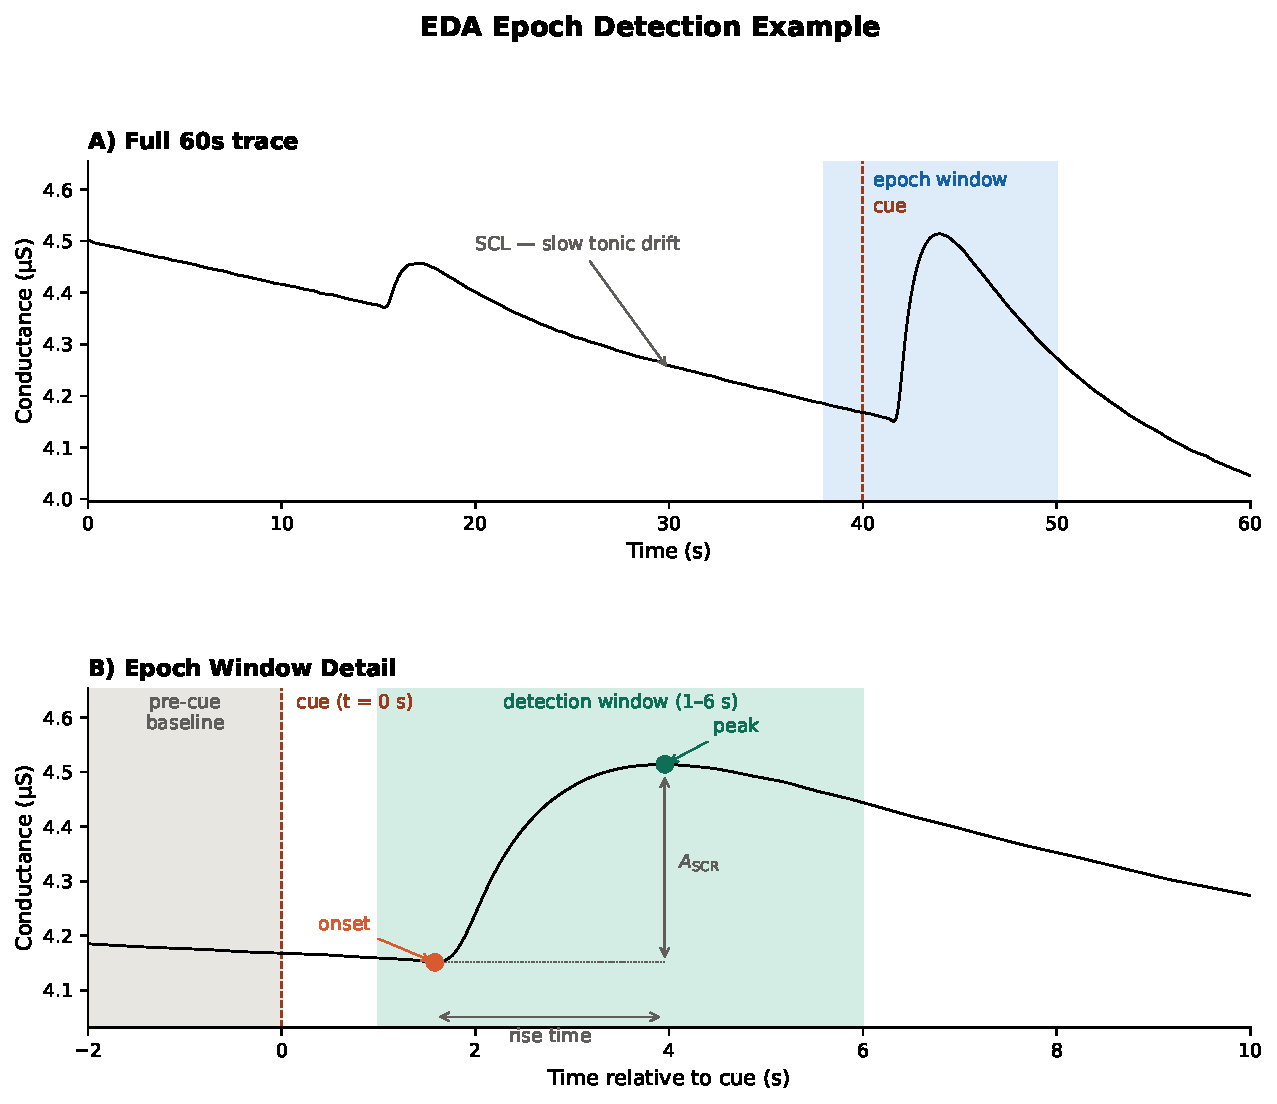
\includegraphics[width=\textwidth]{figures/eda_epoch_figure.pdf}
    \caption{%
        Epoch-based analysis of the EDA signal.
        \textbf{A)} A \SI{60}{\second} segment of the continuous EDA recording, showing the slow tonic drift (SCL) and a stimulus-evoked SCR at the cue event (dashed line). The shaded region marks the extracted epoch.
        \textbf{B)} The extracted epoch referenced to the cue onset. The grey region is the \SI{2}{\second} pre-cue baseline used for per-epoch SCL and local noise floor estimation. The green region is the \SIrange{1}{6}{\second} detection window within which a valid SCR onset must fall. The SCR amplitude $A_\mathrm{SCR}$ is measured from the onset conductance minimum to the response peak. Rise time is the duration from onset to peak. Synthetic data for illustration.
    }
    \label{fig:eda_epoch}
\end{figure}

%Epoch averaging - noise suppression argument for post-isolation signal
The SCR amplitude reported for each block was the mean across all detected epochs within that block. Averaging across stimulus-locked epochs reduced the noise contribution from the isolation stage, since broadband noise is uncorrelated with the stimulus and cancels in the mean, while the physiological response does not.

%EDA SNR - two definitions, circuit and local, diagnostic meaning
Two EDA SNR values were computed per condition using the noise floors defined above. The circuit SNR used the session-level noise floor as the denominator:
\begin{equation}
    \text{SNR}_\text{EDA,circuit} = 20\log_{10}\left(\frac{A_\text{SCR}}{\sigma_\text{baseline,session}}\right)
    \label{eq:eda_snr_circuit}
\end{equation}
The local SNR used the per-epoch noise floor:
\begin{equation}
    \text{SNR}_\text{EDA,local} = 20\log_{10}\left(\frac{A_\text{SCR}}{\sigma_\text{baseline,local}}\right)
    \label{eq:eda_snr_local}
\end{equation}
In both equations, $A_\text{SCR}$ was the mean SCR amplitude across detected epochs within the condition. A gap between the two SNR values within the same condition would indicate that most of the per-epoch noise came from subject activity rather than from the circuit.

The PSD was computed over the full EDA recording using a \SI{10}{\second} window with 50\% overlap, covering the frequency band from \SIrange{0}{1.5}{\hertz}. The window length gave a frequency resolution of \SI{0.1}{\hertz}. A \SI{1}{\second} window produced only two usable bins below \SI{1.5}{\hertz} and could not resolve spectral structure within the EDA band.

Section~\ref{sec:comparative_analysis} describes how these metrics were combined across sessions and conditions to answer Q1-Q7.


\subsection{Comparative Analysis} %What to measure
\label{sec:comparative_analysis}
The validation protocol addressed seven questions, Q1-Q7, each corresponding to a distinct aspect of circuit performance. Questions Q1-Q4 characterized the individual front-ends and the isolation stage separately, while Q5-Q7 evaluated system behavior during simultaneous operation. Tables~\ref{tab:validation_overview_a} and~\ref{tab:validation_overview_b} summarize the sessions, conditions, metrics, and expected figures for each question. The seven questions together provide a comprehensive characterization of the front end, from individual signal quality to cross-circuit interference to session-to-session consistency.
\begin{table}[H]
\centering
\small
\caption{Overview of validation questions Q1-Q4: data sources, metrics, and expected plots.}
\label{tab:validation_overview_a}
\begin{tabular}{P{0.6cm} P{2.2cm} P{2.8cm} P{3.8cm} P{3.8cm}}
\toprule
\textbf{Q} & \textbf{Question} & \textbf{Sessions / blocks} & \textbf{Metrics} & \textbf{Expected plots} \\
\midrule

Q1 & Isolation stage effect &
Sess 1: EMG pre vs post \newline
Sess 2: EDA pre vs post &
\tabitem Attenuation ($X$ = contraction RMS for EMG, mean SCR amplitude for EDA) \newline
\tabitem EMG SNR pre vs post \newline
\tabitem EDA SNR pre vs post (circuit and local) \newline
\tabitem SCR detection rate (EDA) \newline
\tabitem Pearson correlation (pre vs gain-corrected post) &
\tabitem Epoch overlays per condition with means summary (EMG and EDA) \newline
\tabitem PSD overlay: pre vs post (EMG and EDA) \newline
\tabitem SNR bar chart \\
\addlinespace

Q2 & EMG front-end characterization &
Sess 1 post-isolation &
\tabitem Noise floor (mean pre-cue RMS, \si{\micro\volt}) \newline
\tabitem Contraction RMS \newline
\tabitem SNR \newline
\tabitem Mains harmonic power (\SI{50}{\hertz}, \SI{100}{\hertz}, \SI{150}{\hertz}) &
\tabitem Epoch overlay: individual epochs + mean envelope \newline
\tabitem PSD \\
\addlinespace

Q3 & EDA front-end characterization &
Sess 2 post-isolation &
\tabitem SCL \newline
\tabitem Noise floor (session and local) \newline
\tabitem SCR amplitude \newline
\tabitem Rise time \newline
\tabitem Detection rate \newline
\tabitem EDA SNR (circuit and local) &
\tabitem Epoch overlay: individual epochs + mean, onset and peak marked \newline
\tabitem PSD \\
\addlinespace

Q4 & Digital filtering effect &
Sess 1 post-isolation: raw vs filtered &
\tabitem SNR: pre-raw, pre-filtered, post-raw, post-filtered \newline
\tabitem Notch depth at \SI{50}{\hertz} (dB) \newline
\tabitem Mains harmonic power (\SI{50}{\hertz}, \SI{100}{\hertz}, \SI{150}{\hertz}) &
\tabitem Epoch overlays per condition with means summary \newline
\tabitem PSD overlay: all four conditions, notch depth annotated \\

\bottomrule
\end{tabular}
\end{table}

\begin{table}[H]
\centering
\small
\caption{Overview of validation questions Q5-Q7: data sources, metrics, and expected plots.}
\label{tab:validation_overview_b}
\begin{tabular}{P{0.6cm} P{2.2cm} P{2.8cm} P{3.8cm} P{3.8cm}}
\toprule
\textbf{Q} & \textbf{Question} & \textbf{Sessions / blocks} & \textbf{Metrics} & \textbf{Expected plots} \\
\midrule

Q5 & EMG effect on EDA &
Sess 2 EDA-only (clean ref) \newline
Sess 3-5 EDA-only block \newline
Sess 3-5 Combined block &
\tabitem SCL (three-way comparison) \newline
\tabitem SCR amplitude \newline
\tabitem Detection rate \newline
\tabitem EDA SNR (circuit and local) &
\tabitem Epoch overlays per condition with means summary \newline
\tabitem Bar chart: SCL and SNR across three conditions \newline
\tabitem PSD overlay: three conditions ($<$\SI{1.5}{\hertz}) \\
\addlinespace

Q6 & EDA effect on EMG &
Sess 1 EMG-only (clean ref) \newline
Sess 3-5 EMG-only block \newline
Sess 3-5 Combined block &
\tabitem Noise floor \newline
\tabitem Contraction RMS \newline
\tabitem SNR (three-way comparison) \newline
\tabitem PSD low-freq check ($<$\SI{10}{\hertz}) &
\tabitem Epoch overlays per condition with means summary \newline
\tabitem SNR bar chart: three conditions \newline
\tabitem PSD overlay: three conditions ($<$\SI{10}{\hertz}), \SI{3}{\decibel} threshold marked \\
\addlinespace

Q7 & Reproducibility &
Sess 3-5: EMG-only and Combined (EMG); EDA-only and Combined (EDA) &
\tabitem EMG SNR per block (mean$\pm$SD) \newline
\tabitem EDA SCL per block (mean$\pm$SD) \newline
\tabitem EDA SCR amplitude per block (mean$\pm$SD) \newline
\tabitem EDA detection rate per block (mean$\pm$SD) \newline
\tabitem EDA SNR per block (circuit and local, mean$\pm$SD) &
\tabitem Epoch overlays per block, sessions overlaid (EMG and EDA) \newline
\tabitem Bar/box charts: SNR, SCL, SCR amplitude mean$\pm$SD \newline
\tabitem Simultaneous time series: both signals, one contraction + one SCR \\

\bottomrule
\end{tabular}
\end{table}
%Compares signal pre- and post-isolation
%EMG: Session 1, EDA: Session 2
\subsubsection{Q1 - Isolation Stage Effect (EMG and EDA)}
\label{sec:q1}

Q1 evaluated the effect of the galvanic isolation stage on the EMG and EDA signals. Amplitude, frequency content, and waveform morphology were all examined. Data from Session~1 were used for the EMG comparison and data from Session~2 for the EDA comparison. The post-isolation signal was scaled by a factor of three before analysis to compensate for the fixed \nicefrac{1}{3} gain of the ISO224 (Section~\ref{sec:galvanic_isolation}). The Pearson correlation coefficient was computed per epoch between the gain-corrected pre- and post-isolation signals using Equation~\ref{eq:pearson}, over the full epoch window (EMG: \SIrange{-0.5}{3.5}{\second}; EDA: \SIrange{-2}{10}{\second}). The mean and standard deviation were reported across clean epochs for EMG, and across all epochs for EDA. A correlation coefficient near \num{1} would indicate that the isolation stage preserved the waveform shape.

For EMG, attenuation was computed using Equation~\ref{eq:attenuation}, with $X$ defined as the mean contraction RMS across clean epochs. SNR was computed pre- and post-isolation using the mean pre-cue RMS as the noise floor. A preserved SNR across the isolation stage would confirm that the isolator did not degrade the EMG signal. PSD overlays of the pre- and post-isolation signals were inspected to verify that spectral content in the \SIrange{10}{500}{\hertz} band was unchanged.

For EDA, attenuation was computed using Equation~\ref{eq:attenuation} with mean SCR amplitude as $X$. The circuit SNR and local SNR were computed pre- and post-isolation using Equations~\ref{eq:eda_snr_circuit} and~\ref{eq:eda_snr_local}. SCR detection rate was compared pre- and post-isolation to assess whether the isolation stage attenuated phasic responses. Stable SNR and detection rate across the isolation barrier would confirm that the ISO224 did not suppress EDA phasic activity beyond the compensated gain. PSD overlays were inspected to verify that spectral content below \SI{1.5}{\hertz} was preserved.

%Compares baseline vs contraction
%EMG Epoch: -0.5s -> cue -> +3.5s (4s total)
\subsubsection{Q2 - EMG Front-End Characterization}
\label{sec:q2}

Q2 evaluated the signal quality of the EMG front-end during isolated muscle contractions. The post-isolation signal from Session~1 was used, recorded with the EDA circuit physically disconnected. Session~1 contained 120 contraction epochs, each spanning \SIrange{-0.5}{+3.5}{\second} relative to the stimulation cue.

The noise floor was estimated as the mean pre-cue RMS across clean epochs, and the contraction RMS was computed over the 0 to \SI{1.2}{\second} window, following Section~\ref{sec:emg_processing}. SNR was computed as the ratio of contraction RMS to pre-cue RMS in decibels and averaged across all clean epochs using Equation~\ref{eq:snr}. A low noise floor relative to the contraction RMS would indicate that the front-end resolved muscle activity well above the ambient noise level.

PSD was computed over the full Session~1 recording using a \SI{1}{\second} window with 50\% overlap and inspected across the \SIrange{10}{500}{\hertz} band. The mains harmonic power was computed at \SI{50}{\hertz}, \SI{100}{\hertz}, and \SI{150}{\hertz} using Equation~\ref{eq:harmonic_power}. Low total harmonic power and a flat broadband PSD would indicate that the front-end introduced no systematic interference into the signal.

%Compares baseline conductance vs SCR stimulus
%EDA Epoch: -2s -> cue -> +10s (12s total)
%detection window +1-+6s after cue
\subsubsection{Q3 - EDA Front-End Characterization}
\label{sec:q3}

Q3 evaluated the signal quality of the EDA front-end during isolated electrodermal measurement. The post-isolation signal from Session~2 was used, recorded with the EMG circuit physically disconnected. Session~2 contained 30 stimulus epochs, each spanning \SIrange{-2}{+10}{\second} relative to the breath-holding cue.

The SCL, circuit noise floor, and local noise floor were computed following Section~\ref{sec:eda_processing}. SCR amplitude, rise time, and detection rate were extracted from each epoch and averaged across all detected epochs. The circuit SNR and local SNR were computed using Equations~\ref{eq:eda_snr_circuit} and~\ref{eq:eda_snr_local}. A high circuit SNR would indicate that the front-end resolved phasic responses above the hardware noise floor, and a high detection rate would indicate that the SCR threshold was consistently exceeded across trials.

A mean rise time at or above the minimum resolvable limit imposed by the \SI{1.5}{\hertz} analog low-pass filter (\SI{0.67}{\second}) would indicate that the filter constrained the observed SCR dynamics.

PSD was computed over the full Session~2 recording using a \SI{1}{\second} window with 50\% overlap and inspected below \SI{1.5}{\hertz}. A flat noise floor with no dominant spectral peaks in this band would indicate that the front-end introduced no systematic interference into the EDA signal.
%Four signals: pre-isolation raw, pre-isolation filtered, post-isolation raw, post-isolation filtered
%All filtering applied offline via filtfilt on raw data
%Key question: Does the post-isolation filtered approach pre-isolation raw quality?
\subsubsection{Q4 - Digital Filtering Effect (EMG Only)}
\label{sec:q4}

Q4 evaluated how offline digital filtering affected EMG signal quality at both the pre- and post-isolation stages. Four signals were derived from the two raw channels recorded in Session~1: pre-isolation raw, pre-isolation filtered, post-isolation raw, and post-isolation filtered. All digital filtering was applied offline using the filter chain described in Section~\ref{sec:emg_processing}.

The noise floor and SNR were computed for each of the four signals using the mean pre-cue RMS across clean epochs as the noise floor and contraction RMS as the signal amplitude, following Section~\ref{sec:emg_processing}. The notch depth at \SI{50}{\hertz} was computed from the log-ratio of raw and filtered mains harmonic power (Equation~\ref{eq:harmonic_power}) and reported in decibels for each signal. The mains harmonic power was computed at \SI{50}{\hertz}, \SI{100}{\hertz}, and \SI{150}{\hertz} using Equation~\ref{eq:harmonic_power} to quantify how well each harmonic was suppressed. Higher SNR and lower harmonic power in the filtered signals than in the raw signals would indicate that digital filtering recovered signal quality lost to mains interference and broadband noise.

PSD was computed over the full Session~1 recording for all four signals using a \SI{1}{\second} window with 50\% overlap, and the results were inspected across the \SIrange{10}{500}{\hertz} band. Comparing the post-isolation filtered PSD against the pre-isolation raw PSD would indicate whether digital post-processing recovered the spectral quality lost across the isolation barrier.

%Only post-isolated data
%Three-way comparison: Sess2 EDA-only (clean ref) vs Sess3-5 EDA-only vs Sess3-5 Combined
%Compares SCL, SCR amplitude, detection rate, and SNR across conditions
\subsubsection{Q5 - EMG Effect on EDA}
\label{sec:q5}

Q5 evaluated whether simultaneous EMG operation contaminated the EDA signal. Three conditions were compared: Session~2 EDA-only as the clean reference, the EDA-only block from Sessions~3-5, and the Combined block from Sessions~3-5. Metrics were computed per session and averaged across Sessions~3-5. Summary values are reported as mean and standard deviation to convey session-to-session variability. The small sample size (n~=~3 sessions) limited the analysis to descriptive comparison and precluded formal statistical testing.

The SCL was computed as the per-epoch pre-cue mean and compared across all three conditions to detect any tonic offset introduced by simultaneous EMG operation, following Section~\ref{sec:eda_processing}. SCR amplitude, detection rate, circuit SNR, and local SNR were computed for each condition using Equations~\ref{eq:eda_snr_circuit} and~\ref{eq:eda_snr_local}. A shift in SCL between the EDA-only and Combined blocks would indicate that the EMG circuit introduced a tonic offset into the EDA measurement. Stable phasic metrics across conditions would indicate that the galvanic isolation stage prevented EMG interference from reaching the SCR.

PSD was computed for each condition using a \SI{1}{\second} window with 50\% overlap and inspected below \SI{1.5}{\hertz}. Elevated spectral power in the Combined block relative to the EDA-only blocks would indicate residual EMG interference in the EDA frequency band.

%Only post-isolated data
%Three-way comparison: Sess1 EMG-only (clean ref) vs Sess3-5 EMG-only vs Sess3-5 Combined
%Compares noise floor, contraction RMS, SNR, PSD <10Hz across conditions
\subsubsection{Q6 - EDA Effect on EMG}
\label{sec:q6}

Q6 evaluated whether simultaneous EDA operation contaminated the EMG signal. Three conditions were compared: Session~1 EMG-only as the clean reference, the EMG-only block from Sessions~3-5, and the Combined block from Sessions~3-5. Metrics were computed per session and averaged across Sessions~3-5. Summary values are reported as mean and standard deviation to convey session-to-session variability. The small sample size (n~=~3 sessions) limited the analysis to descriptive comparison and precluded formal statistical testing.

The noise floor, contraction RMS, and SNR were computed for each condition using the mean pre-cue RMS across clean epochs as the noise floor, following Section~\ref{sec:emg_processing}. A shift in noise floor or SNR between the EMG-only and Combined blocks would indicate that the EDA excitation current introduced interference into the EMG signal. A stable noise floor and SNR across all three conditions would indicate that the galvanic isolation stage prevented EDA interference from reaching the EMG measurement.

PSD was computed for each condition using a \SI{1}{\second} window with 50\% overlap and inspected below \SI{10}{\hertz}. A mean PSD elevation exceeding \SI{3}{\decibel} across the \SIrange{0}{10}{\hertz} band in the Combined block relative to the EMG-only blocks would indicate EDA-induced low-frequency spectral contamination in the EMG signal.

%Reproducibility across Sessions 3-5
%EMG: EMG-only and Combined blocks. EDA: EDA-only and Combined blocks.
%Metrics reported as mean±SD across three sessions
\subsubsection{Q7 - Reproducibility}
\label{sec:q7}

Q7 evaluated the consistency of simultaneous EMG and EDA measurements across repeated sessions. Data from Sessions~3-5 were used, with all metrics computed per session and reported as mean~$\pm$~standard deviation across the three sessions. The small sample size (n~=~3 sessions) limited the analysis to descriptive comparison and precluded formal statistical testing.

For EMG, the noise floor, contraction RMS, and SNR were reported separately for the EMG-only and combined blocks. A low standard deviation relative to the mean SNR across sessions would indicate that the EMG front-end produced stable signal quality under repeated simultaneous operation. A large deviation would indicate that session-specific factors such as electrode placement or skin preparation dominated the measurement variability.

For EDA, the SCL, SCR amplitude, detection rate, circuit SNR, and local SNR were reported separately for the EDA-only and Combined blocks. A low standard deviation in SCR amplitude and detection rate across sessions would indicate that the EDA front-end consistently resolved phasic responses during repeated simultaneous operation. A large deviation in SCL would indicate habituation differences between sessions rather than circuit instability, since SCL is known to vary with repeated stimulus exposure~\cite{boucsein_electrodermal_2012}.

%Linear Envelope Detection is the most commonly applied demodulation technique used to extract information from the observed EMG waveform.
\begin{itemize}
    \item Describe the methods you use
    \item History
    \item Background
    \item Advantages
    \item Limitations
    \item Applications
    \item What's new?
\end{itemize}

\begin{itemize}
    \item Specifications
    \item Why I chose DC EDA
    \item How does it affect the EMG
    
\end{itemize}